\documentclass[../thesis-main.tex]{subfiles}

\begin{document}

\chapter{Parameter Space Exploration}
\label{ch:paramSpace}

\begin{aquote}{Johannes Brahms}
  {\fontencoding{T1}\fontfamily{pzc}\selectfont
   I sometimes ponder on variation form and it seems to me it ought to be more restrained, purer.
  }
\end{aquote}
\rule{\linewidth}{0.25mm}

\begin{quote}
 \emph{The rationale for using parameter space variation as a means to model physiological variation is presented, with caveats appropriate for this thesis given. Details of which parameters are varied are given, with reasons for their choice. An examination of the efficacy of various different commonly used biomakers as a measure of goodness-of-fit is presented, with a view to determining which biomarkers are most suited under conditions that may include experimental noise. The results of parameter variation for two separate computational model frameworks are explored, and models that reproduce experimentally observed variation are isolated, with patterns amongst the parameters that contribute to these populations being discussed.}
\end{quote}

\section{Reproduction of Experimental Variation}
\label{sec:paramSpace-rationale}
As was elaborated on in \S\ref{sec:param-var}, variation is a constant companion in the experimentalist's world. As computational models of biological processes become more complex, with advancing technology allowing us to discard earlier assumptions made for the sake of computational tractability, and further advances in experimental results allow greater understanding of the system being modelled, variation is now increasingly becoming the computational modeller's companion as well. It is to be noted that this variability includes the so-called experimental variation, the `noise' that can get in the way of the `true' data, but also includes the variation that is a normal, and perhaps essential, component of physiological symptoms.

However, exactly \emph{how} this variation is to be modelled is a question left to the modeller---there are many possible alternatives. Which of these alterantives is to be used depends on the exact question being asked: what system is being modelled, how its output is being assessed, and so forth. It depends further on the available resources, and the demands being made of those resources. Were resources and capabilities infinite and on demand, a fully stochastic, molecular model, subject to multiple simulations, would accurately and precisely model the system---indeed, for all intents and purposes, it would \emph{be} the system. However, not only are resources finite, such a model would be drastic overkill for most research questions regarding cardiac physiology. Instead, much like the research question being posed drives the model choice, it also drives the methodology for reproduction of variability, if it is required---it should be as complex as required, but it need not be any more so.

It is the main drive of this thesis to demonstrate a method for reproducing the observed experimental variation that is
\begin{itemize}
 \item biophysically detailed,
 \item computationally tractable, and
 \item easily scalable.
\end{itemize}
To this end, we utilise the population level approach used previously in neuron modelling \citep{Marder2011}. As compared to stochastic simulations, such a methodology is computationally simpler---due to their complexity and the requirement for multiple simulations for their statistical properties to be refined, stochastic models are often limited to phenomenological, small scale models. This thus ties in to the other advantage of the model population approach: the biophysical detail that can be applied via such a process. In prescribing variation to certain biophysically specific properties, and observing the consequences, specific output variation effects can be attributed to specific input variation effects. It should be noted, however, that \citet{Heijman2013} recently demonstrated the feasibility of using a biophysically-detailed stochastic model, although it is still restricted to small-scale simulations.

Using parallelisation available by means of the Nimrod/G distributed computing grid and its various alternatives, a population model approach is also computationally tractable---each individual simulation can be computationally simple, and correct distribution can ensure that non-specialised computing resources are sufficient to the task. Finally, it is also easily scalable. By this, it is meant that not only is it a simple process to introduce variation to further parameters of interest, but also that the methodology is trivially applicable to multiple models (indeed, this thesis is based on investigations using two different models).

\subsection{Comparison with Alternative Methods}
\label{subsec:alt-methods}
It should be noted that the complete, multi-dimensional parameter sweep method used here provides significant benefits compared to other possible methods, insofar as the goals of this thesis are concerned. By this, it is meant that alternative methods for examining the effect of multiple parameter variation are not appropriate for this thesis. For the purposes of comparison, we may consider three alternative methods:
\begin{enumerate}
 \item Stochastic Models \citep{Heijman2013} \label{list:stochastic}
 \item Multi-variable regression analysis \citep{Sobie2009, Sobie2011, Sarkar2010, Sarkar2011}, \label{list:regression}
 \item Sampling from the multi-dimensional parameter space \citep{Britton2013}, \label{list:multi-sample}
\end{enumerate}
Further details of these methods can be found in \S\ref{subsec:comp-var}. It should be noted that significant work has been achieved using single parameter variation, both in deterministic studies \citep{Romero2009, Romero2011} and in stochastic studies \citep{Pueyo2011, Hashambhoy2011, Sato2009, Tanskanen2005}, but this thesis is explicitly multi-dimensional in scope.

The advantages for this thesis of the population approach over stochastic approaches depends, precisely, on what stochastic approach is being used. In most cases, however, stochastic models are far less computationally tractable, especially for large simulations. This presents limits on the scale of the model that can be simulatted using stochastic means. If one applies stochasticity to multiple parameters (to provide an analogy to the goal of this thesis), the spatial scale of the simulation is curtailed \citep{Heijman2013}. It can also be noted that some studies apply stochasticity within a phenomenological model, but this prevents analysis on the biophysical source of the variability \citep{Walmsley2010}.

Multi-variable regression analysis samples from a given parameter space, and uses this to return the effect matrix $\mathbf{B}$ that approximates the effect each parameter has on a given biomarker \citep{Sobie2009, Sobie2011, Sarkar2010, Sarkar2011}. This methodology is limited by not only sampling from a limited number of models from the total parameter sapce, but also reduces the analysis to a pseudo-single dimensional one---the entries in $\mathbf{B}$ provide insight to the effect of a single parameter on a single output, and it has been demonstrated that the overall effect is relatively accurately approximated by the linear summation of the effects. However, it provides little insight into the interactions between parameters, and especially how these interactions can vary given changes in other parameters (\idest{} parameters $X$ and $Y$ are correlated in a particular manner when parameters $\{A, B, C\}$ have these values, but are correlated in a different manner when $\{A, B, C\}$ have different values).

Methodologically, the most similar method to the current is to sample from the multi-dimensional space to generate a population. This was done by \citep{Davies2012}, but only generated a population of 19 models for a canine ventricular AP. The work previously mentioned by \citet{Britton2013} presents the most comprehensive study in cardiac studies. However, sampling from the multi-dimensional space likely gives an incomplete picture, and is thus less suited to analyse the effects of multiple parameter variation. While it does present a computationally efficient means of population production, it should be noted that (a) it may be unable to give a comprehensive account of the parameter variation within the space and (b) \citet{Gemmell2010a} suggests that there may be `islands' within the population, and insufficient sampling will either miss these islands, or falsely connect them with nearby groups in the parameter space; further consideration of these problems is given in \S\ref{subsec:space-connectivity}).

\subsection{Caveats}
\label{subsec:caveats}
It should be noted that constructing a population of models based on a single framework (replacing the initial parameter set with a parameter space) allows for a biophysically realistic method of reproducing physiological variation which remains computationally tractable. However, there are several key points that must be remembered that represent the limitations of this, and many related, approach.
\begin{enumerate}
 \item The underlying assumptions regarding the original model still apply. As such, any inaccurate assumptions remain present in derived populations \citet{Noble2001, Quinn2013}.
 \item The populations derived using experimental data rely on these data remaining appropriate for the considered task. The populations used in this thesis are derived using `healthy' data. As such, without further adaptation, the populations are unsuitable for assessing some experimental situations without appropriate alterations made to the framework, \eg{} where cardiac remodelling has occurred \citep{Walmsley2013}.
 \item Related to the point above is the fact that the model populations are united by the data used to create them. As such, if the training data used include differences such as gender, the models cannot then be used to address specific questions regarding gender---these differences are now implicitly encoded within the population.
\end{enumerate}

For this dissertation, cell models are being used, but tissue data are being used for training the population. Moving from cell to tissue represents a large computational task, for two reasons. Firstly, the simple matter of simulating tissue is more computationally intensive, though preliminary simulations using the original Shannon model indicated little difference between the AP generated using cell simulations and those from tissue simulations (performed using the Chaste software \citep{Mirams2013}). Secondly, and more pertinent for this thesis, is the problem of cell coupling (which itself is a likely candidate for variation). \citet{Heijman2013} predict that cell coupling works to reduce variation between two different cells---by this token, it is likely that any cell model population trained using tissue data is likely to represent an underestimate of the actual variation possible within a cell population. However, to exhaustively test this is computationally challenging. Consider the following: suppose it is wished to test just 20 different cells. To exhaustively examine every possible combination of this population in a 2 cell chain, it would be required to perform $20^2$. It is simple to abstract this---for a possible cell population of $n$, in a tissue sample of size $m$, the number of simulations that would have to be run would be $n^m$. While there are many possible ways to reduce the search space, it is beyond the scope of this thesis to consider them.

Finally, there is a caveat common to almost all attempts to reproduce variation; indeed, it can be applied to most models as well. \citet{Walmsley2013} demonstrated little correlation between AP and \ca{} biomarkers---this will be expanded upon in \S\ref{sec:param-effects}.

\section{Construction of the Parameter Space}
\label{sec:paramSpace-methods}
The computational tools involved in investigating the effects of multiple parameter variation were described in the previous chapter---the specific methods used to that end and biological reasons for these methods are described here.

Parameters describing the peak conductance for six different ion channels were varied in this study. The currents considered (with their conductance given in parentheses) were: the transient outward current (\gto{}), the rapid delayed rectifier \K{} current (\gkr{}), the slow delayed rectifier \K{} current (\gks{}), the inward rectifying \K{} current (\gkix{}), the L-tpye \ca{} current (\gca{}), and the \na{}/\K{} pump current (\gnak{}). These currents were picked in preference to other possible choices based on their perceived impact on the repolarisation of the AP, which has been noted as an indicator of impact on beat-to-beat variability of repolarisation duration (BVR); a longer plateau implies greater BVR \citep{Heijman2013}. Furthermore, the dynamics of these currents were not changed on the basis that (a) it was expected that AP variability is primarily a result of differences in the relative magnitude of the currents rather than the dynamics, and (b) conductance is often the most poorly defined variable within the equations defining these currents in the models. This difficulty in parameter estimation comes from both the inherent experimental difficulties in measuring peak conductance, and the variation in the experimental techniques used to define these values (with methods sometimes being poorly defined) \citep{Quinn2011}.

The conductances were varied by $0\%$, $\pm15\%$, and $30\%$, resulting in 15,625 different models for each framework. This variation is in line with the extent of variation used in previous studies \citep{Romero2009, Romero2011, Walmsley2013}, and is also consistent with the range of experimentally observed variation \citep{Fulop2004, Iost1998, Li1999, Szentadrassy2005, Verkerk2005, Sims2008} (for further detail, see \S\ref{sec:param-var}). While some computational studies have used greater degrees of variation, it was decided the variation applied here provided the best compromise between scale and resolution of the parameter space. Furthermore, variation of such scale is not often seen in experimental literature.

Simulations were conducted a three different cycle lengths (CLs) of 400 ms, 600 ms and 1,000 ms to constrain the population of models further---\citet{Syed2005} has demonstrated the importance of considering multiple CLs in order to accurately fit restitution curves. Furthermore, this methodology allows examination of rate-dependent effects, \eg{} changing parameter importance, changing degrees of output variation.

\section{Accuracy of Biomarkers in Defining Model Fit}
\label{sec:biomarker-accuracy}
One of the goals of this thesis is to measure the efficacy of commonly used biomarkers in assessing goodness-of-fit for populations. With a parameter sweep providing a population of models, and thus a population of data, that is free from experimental noise, this provides an opportunity for an assessment of such a question. Without having to consider the problems of experimental noise, the entire range of recorded data can be used to compare a given model output to given training data. The goodness-of-fit by this comprehensive measure can then be compared to the goodness-of-fit given by other biomarkers.

In this specific case, the NRMSD metrics defined in \S\ref{sec:biomarkers} were used to compare the output of any given model to the output of the original, unaltered model (\idest{} the model with $0\%$ variation for all parameters). As previously stated, $M_\textnormal{NRMSD}$ is unsuited to situations with experimental noise, but in situations where there is no computational noise (as in this parameter search), it provides a comprehensive measure of goodness-of-fit. On the assumption that, due to its involving the totality of available data, it provides the `best' measure of goodness-of-fit, it it is then possible to assess how closely other biomarkers come to agreeing with this new gold standard; those biomarkers that come closest to defining the same models as the NRMSD metrics as `matching' training data will then be considered accurate measures of goodness-of-fit in their own right.\footnote{It can be noted that, for cells with a long diastolic interval, small differences in \vrest{} would increase \aprms{} to a great degree, while the rest of the AP may provide an excellent fit to data. Fortunately, both Shannon and Mahajan populations show little variation in \vrest{}, so this problem is not realised} This process uses multiple biomarkers in unison, \eg{} APD\sub{50} and APD\sub{90}, rather than individual biomarkers in isolation.

The $\sim250$ models most closely matching the original model output were determined, based on the minimum values of $M_\textnormal{NRMSD}$. Similarly, the $\sim250$ models that match original model output was determined based on minimum percentage difference according to groups of biomarkers. The degree of overlap between these two groups (those determined by NRMSD metrics and those determined by biomarkers) was then calculated.

The results of the comparison for some biomarker groups is shown in Fig.~\ref{fig:biomarker-compare}. When \cai{} data is available, and thus \ca{} biomarkers can be used in assessing the goodness-of-fit, the accuracy (judged by percentage overlap) is increased overall. The degree of overlap for groups of metrics is not identical between the Shannon and Mahajan populations. However, overall, a combination of APD\sub{50}, APD\sub{90} and CaT (or APD\sub{50} and APD\sub{90} where \cai{} data are not available), is the most accurate measure of goodness-of-fit compared to NRMSD metrics. Consequently, these combinations were used for the remainder of this thesis.
\begin{figure}
 \centering
 \includegraphics[width=0.7\textwidth]{biomarker-compare}
 \caption[Efficacy of biomarkers in determining goodness-of-fit.]{Percentage overlap of matches between original model output and model output generated using the $\sim250$ parameter sets determined by the NRMSD metrics ([\aprms{} and \carms{}]) and by combinations of biomarkers. While all combinations of biomarkers were tested, those shown represent the combinations with the highest percentage overlap. Combinations to the left of the dashed line include information about both $V_m$ and \cai{}, while those to the right include only $V_m$ data.}
 \label{fig:biomarker-compare}
\end{figure}

\section{Defining a Population of Models to Reproduce Physiological Variation}
\label{sec:population}

\subsection{Variation within the Population}
\label{subsec:population-trends}
In order to constrain the populations of models to those representing physiological variability, only parameter sets that produced APD\sub{50} and APD\sub{90} values that fell within the normal range for rabbit epicardium were included. APD\sub{90} for rabbit epicardium has been well documented and a physiological range was readily established for all CLs \citep{Biagetti2006, Chen2006, Eckardt1998, Goldhaber2005, Jung2011, Kirchhof2003, Kurz1993, McIntosh2000, Szigligeti1996, Wu2011, Yan2001}. Reports of APD\sub{50} values sufficient to derive a normal range, however, were not available at all CLs. Thus, values from the literature were used to establish a mean value for APD50 \citep{Eckardt1998, Kirchhof2003}. It was then assumed that the percentage variation from mean for APD\sub{50} is the same as the percentage variation from mean for APD\sub{90}. By this assumption, an assumed range for APD\sub{50} that is similar to the range for APD\sub{90} is calculated, and used in subsequent analysis. The resulting values are shown in Table~\ref{table:physiological-range}.
\begin{table}
 \centering
 \begin{tabular}{c|ccc}
  \multirow{2}{*}{Biomarker} & \multicolumn{3}{|c}{CL (ms)} \\
  & 400 & 600 & 1,000 \\
  \hline
  \hline
  APD\sub{50} (ms) & $104-135$ & $116-159$ & $137-188$ \\
  APD\sub{90} (ms) & $142-185$ & $160-220$ & $167-230$
 \end{tabular}
 \caption[Physiological Ranges for APD\sub{50} and APD\sub{90}]{Normal range of rabbit epicardial APD\sub{50} and APD\sub{90} used to define physiological parameter sets. Values are derived from previously reported studies, as described in the text.}
 \label{table:physiological-range}
\end{table}

By using these values, it was possible to constrain the tested parameter space to a population of models that reproduces experimentally measured variability at each CL. The number of models in each population at each CL is given in Table~\ref{table:population-numbers}. Those models that produce output within the physiological range are defined to be in the model population that can reproduce given variation at all CLs; the minimum, mean and maximum values of all computed biomarkers for the Shannon and Mahajan populations thus defined are shown in Table~\ref{population-minMeanMax}.
\begin{table}
 \centering
 \begin{tabular}{c|ccccccc}
  \multirow{2}{*}{Model} & \multicolumn{7}{|c}{CL (ms)} \\
  & 400 & 600 & 1,000 & 400$\cap$600 & 400$\cap$1,000 & 600$\cap$1,000 & 400$\cap$600$\cap$1,000 \\
  \hline
  \hline
  Shannon & 1,691 & 2,631 & 5,352 & 1,384 & 1,511& 2,526 & 1,352 \\
  Mahajan & 3,946 & 1,031 & 0 & 577& 0 & 0 & 0 \\
  Expanded Mahajan & 9,447 & 11,229 & 5,650 & 6,797 & 779 & 4,331 & 779
 \end{tabular}
 \caption[Number of parameter sets producing both APD\sub{50} and APD\sub{90} values within the physiological range.]{Number of parameter sets producing both APD\sub{50} and APD\sub{90} values within the physiological range. Parameter values were varied by $\pm30\%$ from the original parameter set, and then further for the Mahajan model (`Expanded Mahajan') as explained in the text. $x \cap y$ and $x \cap y \cap z$ represent parameter sets that produce physiological values at a CL of $x$ and $y$, or a CL of $x$, $y$, and $z$, respectively.}
 \label{table:population-numbers}
\end{table}

\begin{table}
 \centering
 \begin{tabular}{cccccc}
  Biomarker & CL (ms) & Model & Minimum & Mean & Maximum \\
  \hline
  \hline
  \multirow{4}{*}{\dvdtmax{} (Vs$^{-1}$)} & \multirow{2}{*}{400} & Shannon & $233$ & $302$ & $329$ \\
  & & Mahajan & $200$ & $230$ & $252$ \\
  & \multirow{2}{*}{1,000} & Shannon & $278$ & $327$ & $352$ \\
  & & Mahajan & $248$ & $279$ & $311$ \\
  \hline
  \multirow{4}{*}{\vrest{} (mV)} & \multirow{2}{*}{400} & Shannon & $-92$ & $-88$ & $-82$ \\
  & & Mahajan & $-88$ & $-86$ & $-85$ \\
  & \multirow{2}{*}{1,000} & Shannon & $-88$ & $-86$ & $-81$ \\
  & & Mahajan & $-89$ & $-88$ & $-87$ \\
  \hline
  \multirow{4}{*}{APD\sub{50} (ms)} & \multirow{2}{*}{400} & Shannon & $112$ & $126$ & $135$ \\
  & & Mahajan & $104$ & $108$ & $117$ \\
  & \multirow{2}{*}{1,000} & Shannon & $137$ & $155$ & $181$ \\
  & & Mahajan & $165$ & $182$ & $188$ \\
  \hline
  \multirow{4}{*}{APD\sub{90} (ms)} & \multirow{2}{*}{400} & Shannon & $143$ & $154$ & $169$ \\
  & & Mahajan & $142$ & $155$ & $185$ \\
  & \multirow{2}{*}{1,000} & Shannon & $167$ & $186$ & $217$ \\
  & & Mahajan & $207$ & $223$ & $230$ \\
  \hline
  \multirow{4}{*}{\cadia{} ($\mu$M)} & \multirow{2}{*}{400} & Shannon & $1.24$ & $1.29$ & $1.32$ \\
  & & Mahajan & $0.29$ & $0.37$ & $0.47$ \\
  & \multirow{2}{*}{1,000} & Shannon & $0.82$ & $0.84$ & $0.86$ \\
  & & Mahajan & $0.15$ & $0.16$ & $0.18$ \\
  \hline
  \multirow{4}{*}{\casys{} ($\mu$M)} & \multirow{2}{*}{400} & Shannon & $4.49$ & $4.92$ & $5.22$ \\
  & & Mahajan & $1.43$ & $2.78$ & $4.46$ \\
  & \multirow{2}{*}{1,000} & Shannon & $3.13$ & $3.33$ & $3.68$ \\
  & & Mahajan & $0.41$ & $0.59$ & $0.76$ \\
  \hline
  \multirow{4}{*}{CaT ($\mu$M)} & \multirow{2}{*}{400} & Shannon & $3.25$ & $3.63$ & $3.91$ \\
  & & Mahajan & $1.14$ & $2.41$ & $4.00$ \\
  & \multirow{2}{*}{1,000} & Shannon & $2.30$ & $2.49$ & $2.82$ \\
  & & Mahajan & $0.26$ & $0.42$ & $0.58$ \\
  \hline
  \multirow{4}{*}{CTD\sub{50} (ms)} & \multirow{2}{*}{400} & Shannon & $123$ & $130$ & $134$ \\
  & & Mahajan & $133$ & $139$ & $147$ \\
  & \multirow{2}{*}{1,000} & Shannon & $139$ & $150$ & $157$ \\
  & & Mahajan & $208$ & $231$ & $268$ \\
  \hline
  \multirow{4}{*}{CTD\sub{90} (ms)} & \multirow{2}{*}{400} & Shannon & $263$ & $267$ & $271$ \\
  & & Mahajan & $245$ & $249$ & $260$ \\
  & \multirow{2}{*}{1,000} & Shannon & $382$ & $394$ & $404$ \\
  & & Mahajan & $460$ & $510$ & $585$ \\
 \end{tabular}
 \caption[Minimum, mean, and maximum values of all computed biomarkers produced with the physiological parameter sets.]{Minimum, mean, and maximum values of all computed biomarkers produced with the physiological parameter sets.}
 \label{table:population-minMeanMax}
\end{table}

With the Shannon framework, there existed at least one parameter set that produced a physiological output at each CL, with some of these generating a physiological output at all CLs. On the other hand, while a relatively large number of models produced a physiological output at a CL of 400 ms with the Mahajan framework (the CL for which the original Mahajan model was designed), fewer parameter sets matched at a CL of 600 ms, and none at a CL of 1,000ms (the increase in APD with increasing CL was disproportionately large).

In order to address the failure of the Mahajan framework in finding parameter sets that generated a physiological output with increased CL, the range of conductance variation was expanded. To determine the direction of this expansion, the first step was to increase the ranges of APD\sub{50} and APD\sub{90} by $\pm10\%$, and the parameter space was compared to this new range. This expanded range of APD resulted in `matches' being found at all CLs. Based on the trends in the conductances evident amongst these matches, the parameter ranges were altered and a new parameter space was explored. The new ranges are shown in Fig.~\ref{fig:expandedMahajan}, and resulted in an additional 15,625 models being simulated. However, even with this expanded search, the number of parameter sets that matched at all CLs was approximately half of that with the Shannon model.
\begin{figure}
 \centering
 \includegraphics[width=0.7\textwidth]{expandedMahajan}
 \caption[Parameter ranges used For `Expanded Mahajan' search.]{Parameter ranges used For `Expanded Mahajan' search.}
 \label{fig:expandedMahajan}
\end{figure}

The parameter sets producing a physiological output with the Shannon framework are shown using a dimensional stack in Fig.~\ref{fig:shannon-population}, along with the generated $V_m$ and \cai{} profiles at a CL of 400 and 1,000 ms, and the associated distribution of conductance values. The most obvious trend is that parameter sets producing a physiological output generally had a simultaneous reduction in both \gca{} and \gkix{}. This is evident in both Fig.~\ref{fig:shannon-population}A, demonstated by a clustering of the valid models at the bottom left of the dimensional stack, and from the associated distribution of conductances, shown in Fig.~\ref{fig:shannon-population}D. It also appears that the distribution of the other conductances was fairly even; however, a closer examination of the dimensional stack in Fig.~\ref{fig:shannon-population}A reveals trends between the parameters (demonstrating the power of the clutter-based dimension reordering technique for visualisation of multi-dimensional parameter spaces). For instance, within the \gnak{}/\gkr{} surfaces (Level 2 of the stack), the matching parameter sets are spread in an approximately diagonal line from top left to bottom right, indicating that when \gnak{} was increased, this was offset by a decrease in \gkr{}, and \emph{vice versa}. As \gca{} and \gkix{} decrease, this diagonal line moves further to the bottom left corner, indicating that a further reduction of \gnak{} and \gkr{} was required to continue to produce a physiological output.
\begin{figure}
 \centering
 \includegraphics[width=0.7\textwidth]{shannon-population}
 \caption[Model population for the Shannon framework that produces values of both APD\sub{50} and APD\sub{90} that fall within the experimentally derived range.]{Model population for the Shannon framework that produces values of both APD\sub{50} and APD\sub{90} that fall within the experimentally derived range. (A) Dimensional stack image showing the location of matching parameter sets for each CL and their overlap. (B) $V_m$ and \cai{} (inset) profiles for the matching parameter sets at a CL of 400 ms. (C) $V_m$ and \cai{} (inset) profiles for the matching parameter sets at a CL of 1,000 ms. (D) Distribution of conductance values for the valid parameter sets. For both (B) and (C), the physiological ranges of APD\sub{50} and APD\sub{90} are represented by the blue and red rectangles, respectively.}
 \label{fig:shannon-population}
\end{figure}

The effect of \gto{} is more complicated. When \gca{} and \gkix{} were reduced by $30\%$, and \gnak{} was also reduced, matching parameter sets then included those with an increased \gto{}. The opposite was true when \gnak{} was increased, as in these cases a decrease in \gto{} was necessary (square A1 in Fig.~\ref{fig:shannon-population}A). As \gkix{} was increased, fewer parameter sets with an increased \gnak{} were valid, such that an increase in \gto{} was observed (squares B1, C1, and D1 in Fig.~\ref{fig:shannon-population}). However, in all cases where \gca{} was not reduced by $30\%$, the opposite was true: parameter sets included reduced \gnak{} and increased \gto{} were no longer valid (squares A2 and A3 in Fig.~\ref{fig:shannon-population}). Finally, in all valud parameter sets as \gkix{} was increased, \gto{} decreased. On the other hand, there appeared to be no pattern to the values of \gks{} within the model population.

For the expanded Mahajan search, the parameter sets producing a physiological output, the generated cellular profiles, and the distribution of valid conductance values are shown in Fig.~\ref{fig:mahajan-population}. There are some differences compared to the Shannon framework. For instance, with the Shannon framework, \gks{} appeared to have no effect in determining the validity of parameter sets, while with the Mahajan framework it had a strong influence, as most matching parameter sets included the largest conductance variation ($+105\%$). The opposite was true for \gkix{}: while it had a large influence with the Shannon framework, it was relatively unimportant with the Mahajan framework. Similarly, with the Shannon framework, \gto{} and \gnak{} generally varied in the opposite direction, while with the Mahajan framework they changed in the same direction.
\begin{figure}
 \centering
 \includegraphics[width=0.7\textwidth]{mahajan-population}
 \caption[Model population for the expanded Mahajan framework that produces values of both APD\sub{50} and APD\sub{90} that fall within the experimentally derived range.]{Model population for the expanded Mahajan framework that produces values of both APD\sub{50} and APD\sub{90} that fall within the experimentally derived range. (A) Dimensional stack image showing the location of matching parameter sets for each CL and their overlap. (B) $V_m$ and \cai{} (inset) profiles for the matching parameter sets at a CL of 400 ms. (C) $V_m$ and \cai{} (inset) profiles for the matching parameter sets at a CL of 1,000 ms. (D) Distribution of conductance values for the valid parameter sets. For both (B) and (C), the physiological ranges of APD\sub{50} and APD\sub{90} are represented by the blue and red rectangles, respectively.}
 \label{fig:mahajan-population}
\end{figure}

With the Mahajan model, there was also a strong correlation between \gnak{} and \gks{}, such that when \gnak{} was increased, \gks{} also increased (demonstrated by a shift of mathcing parameter sets from the predominantly lower left corner to the upper right corner of the level two plots in Fig.~\ref{fig:mahajan-population}A; for instance, compare the distribution within E1 and E3). On the other hand, there appeared to be no limitations on the values of \gkr{}.

It is of note that the original model for both frameworks is not included in the final model populations. This does not in any way remove the validity of these models---they are entirely valid for the CLs for which they were designed. It can also be compared to \citet{Sato2009}, in which different parameters had to be used within the model to generate the required behaviour. However, this does demonstrate the limitations of any given model, and the requirement to be careful of any applications for which the model/framework was not explicitly designed. On a related note, it can be observed that there is little variation observed in \vrest{} in both populations. While this is almost to be expected (none of the varied parameters would be expected to have a great effect on this biomarker), it should be noted that, in experimental data, \vrest{} is rarely so well-behaved.

While the results presented here suggest that variation in current conductances over a wide range of values may account for normal variability in rabbit ventricular AP repolarisation, other factors may be involved. One of the underlying assumptions of this thesis is that AP variability is primarily a result of differences in the relative magnitude of the currents, rather than underlying current dynamics, which were not varied. Changes in channel properties other than conductance could result in similar changes in AP biomarkers, and also account for some of the experimentally observed variability. \citet{Romero2011} presented a one-dimensional sensitivity analysis of the rabbit-specific frameworks used in this thesis with a similar range of parameter variation, and showed that along with repolarisation currents, APD was significantly modified by changes in the activation and inactivation rates of the associated channels. At the same time, further constraints to the model populations (\eg{} matching of rate-adaptation of restitution properties), as well as consideration of additional biomarkers (for instance, relating to intracellular ion concentration), may be necessary to ensure their applicability to additional physiological states. This has been recently demonstrated in \citet{Walmsley2013}, in which populations of failing and non-failing human ventricular myocytes with variation in current conductances were compared using various biomarkers at numerous CLs to investigate which currents drive variability in the two cell populations. Finally, as the range and resolution of parameter space sampling in teh present study was limited by computational tractability, there may be additional influences and interactions of current conductances important for ventricular AP variability that were not appreciated. As mentioned earlier, it is difficulat to properly asses the true physiological ranges of the current conductances considered in this study, so that they may be related to the values included in the calibrated populations of models. We initially varied all conductances by $\pm30\%$, yet it was necessary with the Mahajan framework to expand this range to generate a physiological output. Other computational studies have used a larger range of conductances than presented here \citep{Sobie2009, Britton2013, Davies2012}, possibly representing the true physiological range of values, and supporting the expanded range used with the Mahajan framework..

\subsection{Connectivity within the Parameter Space}
\label{subsec:space-connectivity}
Of note is the question which has been touched upon earlier, both in this study and others: are the populations generated here `connected', by which it is asked whether or not one can connect all models in the population with a single parameter space, or does the population consist of several separate populations within the population space. The answer to this is irritatingly dependent on how, exactly, one defines `connected'. If one requries connection only by one step in multiple dimensions, then the populations derived here are connected. However, if one adopts a stricter definition of connection (two models are connected only if they are one step away from each other in a single dimension), then the populations are not connected---this is shown in a dimensional stack in Fig.~\ref{fig:space-connectivity}.
\begin{figure}
 \centering
 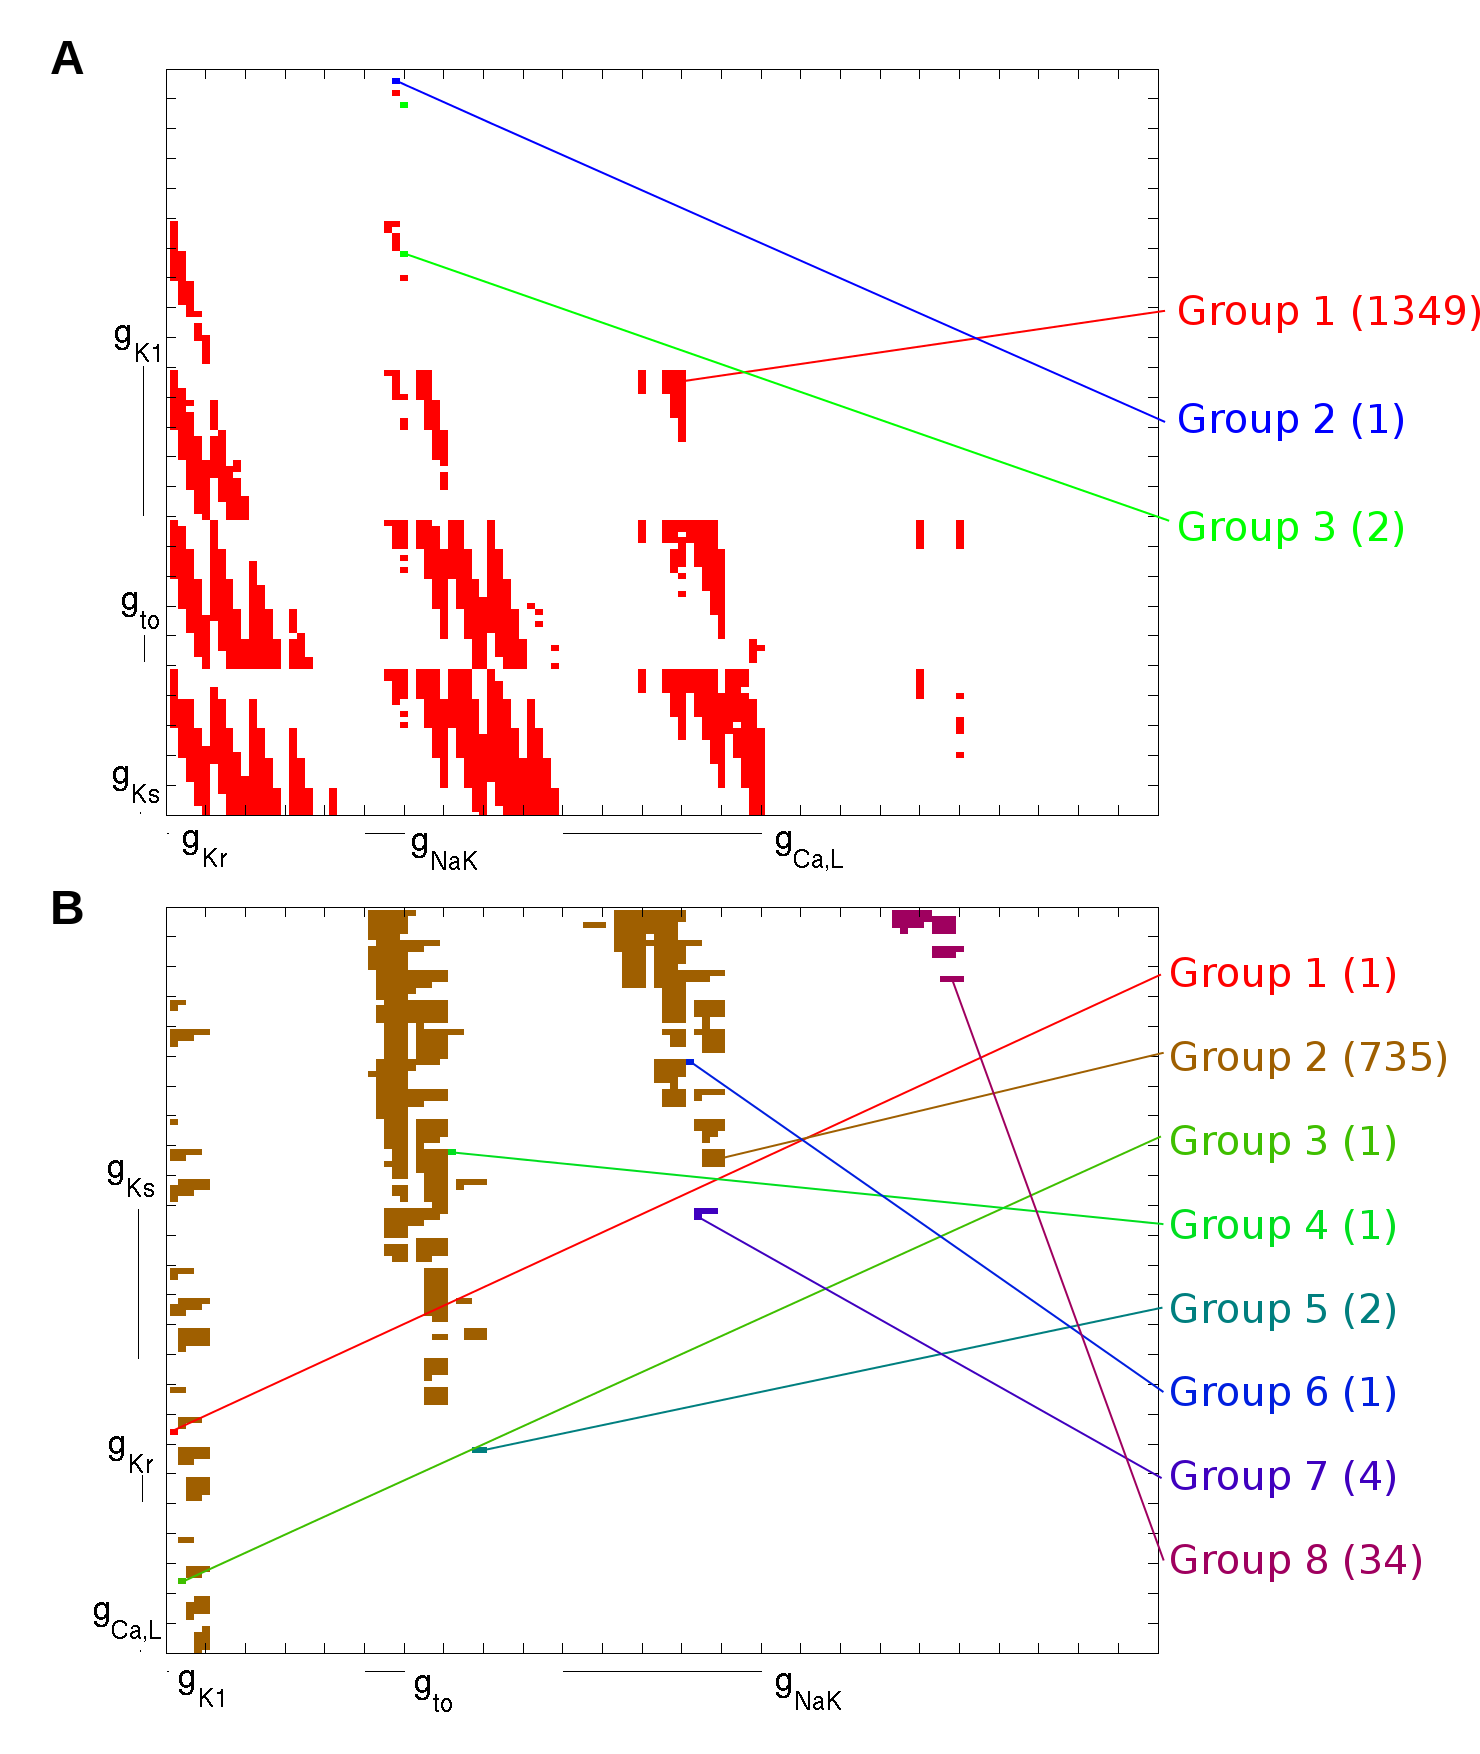
\includegraphics[width=0.7\textwidth]{space-connectivity}
 \caption[Connectivity within model populations.]{Dimensional stack images showing connectivity within model populations for the Shannon (A) and Mahajan (B) frameworks, with a space defined as being connected if two points are connected only if they are one step away from each other in a single dimension. The numbers within the parentheses represent the number of models within each group.}
 \label{fig:space-connectivity}
\end{figure}

It is beyond the scope of this thesis to determine whether the two definitions of connectivity can be reconciled---whether by increased resolution, or by inclusion of alternative parameters, those semi-connected regions will become connected. However, if we work on the (somewhat reasonable) assumption that either they can, or the looser defintion of connectivity is a reasonable approximation, this has significant implications for population construction, in that it implies that, once a `valid' model has been found, the search for other `valid' models can be directed, and thus the computational task of searching the entire parameter space is reduced.

\section{Effects of Parameter Variation}
\label{sec:param-effects}
Using the biomarkers thus defined as providing measures of goodness-of-fit, it is now possible to assess the effects of parameter variation on the model populations; it also allows judgement of how these different biomarkers are affected by these different parameters, and how these differences are altered based on CL. The dimensional stack images showing these effects are presented in Fig.~\ref{fig:shannon-paramEffect} (for the Shannon population) and Fig.~\ref{fig:mahajan-parameffect} (for the Mahajan population). In addition, the optimum stack orders are shown in Table~\ref{table:optimum-order}.
\begin{figure}
 \centering
 \includegraphics[width=\textwidth]{shannon-paramEffect}
 \caption[Effect of parameter variation on Shannon population.]{Dimensional stack images demonstrating the effect of simultaneously varying the magnitude of six repolarising current conductances in the Shannon model. The top, middle, and bottom rows show the effects on APD\sub{50}, APD\sub{90}, and CaT, respectively. The left column is based on simulations with a CL of 400 ms and the right with a CL of 1,000 ms. In the contour plots, red represents an increase from the initial parameter value, blue a decrease, and white no change. The physiological range determined from the literature (see \S\ref{sec:population} for details) is represented by the grey region next to the colour bars in each panel. Black dots represent parameter sets with which the model did not reach steady state. In this case the optimum stack orders are not displayed; instead the order before optimisation has been used, which allowed direct comparison of the stacks to reveal differences in effects on each biomarker.}
 \label{fig:shannon-paramEffect}
\end{figure}

\begin{figure}
 \centering
 \includegraphics[width=\textwidth]{mahajan-paramEffect}
 \caption[Effect of parameter variation on Mahajan population.]{Dimensional stack images demonstrating the effect of simultaneously varying the magnitude of six repolarising current conductances in the Mahajan model. The top, middle, and bottom rows show the effects on APD\sub{50}, APD\sub{90}, and CaT, respectively. The left column is based on simulations with a CL of 400 ms and the right with a CL of 1,000 ms. In the contour plots, red represents an increase from the initial parameter value, blue a decrease, and white no change. The physiological range determined from the literature for a CL of 400 ms is represented by the grey region next to the colour bars in each panel (the grey region is absent for a CL of 1,000 ms as the APD values fell outside of the physiological range). In this case the optimum stack orders are not displayed; instead the order before optimisation has been used, which allows direct comparison of the stacks to reveal differences in effects on each biomarker.}
 \label{fig:mahajan-paramEffect}
\end{figure}

\begin{table}
 \centering
 \begin{tabular}{ccc|ccc}
  \multirow{2}{*}{Framework} & \multirow{2}{*}{Biomarker} & \multirow{2}{*}{CL (ms)} & \multicolumn{3}{|c}{Optimum Stack Order $(x,y)$} \\
  & & & \multicolumn{3}{|c}{Low Order $\longrightarrow$ High Order} \\
  \hline
  \hline
  \multirow{6}{*}{Shannon} & \multirow{2}{*}{APD\sub{50}} & 400 & (\gto{},\gks{}) & (\gnak{},\gkr{}) & (\gca{},\gkix{}) \\
  & & 1,000 & (\gkix{},\gks{}) & (\gnak{},\gkr{}) & (\gca{},\gto{}) \\
  \cline{2-6}
  & \multirow{2}{*}{APD\sub{90}} & 400 & (\gto{},\gks{}) & (\gnak{},\gkr{}) & (\gca{},\gkix{}) \\
  & & 1,000 & (\gkix{},\gks{}) & (\gnak{},\gkr{}) & (\gca{},\gto{}) \\
  \cline{2-6}
  & \multirow{2}{*}{CaT} & 400 & (\gkix{},\gks{}) & (\gnak{},\gto{}) & (\gca{},\gkr{}) \\
  & & 1,000 & (\gkix{},\gks{}) & (\gnak{},\gkr{}) & (\gca{},\gto{}) \\
  \hline
  \multirow{6}{*}{Mahajan} & \multirow{2}{*}{APD\sub{50}} & 400 & (\gkr{},\gkix{}) & (\gks{},\gca{}) & (\gto{},\gnak{}) \\
  & & 1,000 & (\gkr{},\gkix{}) & (\gto{},\gca{}) & (\gks{},\gnak{}) \\
  \cline{2-6}
  & \multirow{2}{*}{APD\sub{90}} & 400 & (\gkr{},\gca{}) & (\gkix{},\gks{}) & (\gto{},\gnak{}) \\
  & & 1,000 & (\gkr{},\gkix{}) & (\gks{},\gto{}) & (\gca{},\gnak{}) \\
  \cline{2-6}
  & \multirow{2}{*}{CaT} & 400 & (\gkr{},\gkix{}) & (\gto{},\gks{}) & (\gnak{},\gca{}) \\
  & & 1,000 & (\gkr{},\gkix{}) & (\gks{},\gto{}) & (\gnak{},\gca{}) \\
 \end{tabular}
 \caption[Optimum stack order for APD\sub{50}, APD\sub{90}, and CaT for the Shannon and Mahajan frameworks]{Optimum stack order for APD\sub{50}, APD\sub{90}, and CaT for the Shannon and Mahajan frameworks, at CLs of 400 and 1,000 ms. Each pair of parameters represents low, medium, or high order current conductances. For each pair, the first component is plotted on the x-axis and the second component on the y-axis. The $(x,y)$ order can be reversed without affecting the result, though only if \emph{all} $(x,y)$ pairs are reversed.}
 \label{table:optimum-order}
\end{table}

These results demonstrate how the relative importance of the varied current conductances was dependent on both the CL, and on the biomarker being considered. In considering this, it should be noted that the non-linear interactions between currents and ion concentrations often resulted in different changes in the current magnitudes that might be expected from the change in current conductance. For instance, when \gks{} was subject to $\pm30\%$ variation at a CL of 1,000 ms, the amplitude of \iks{} varied from $-99\%$ to $+386\%$ for the Mahajan population. \todo{CHECK THE DETAILS OF THIS MORE PRECISELY}.

The optimum stack order, which is an indication of both the relative importance of the individual conductances on the biomarker and the inter-relation between parameters, changes with CL. The extent of this change is unpredictable, and can be dramatic. This is best demonstrated with the Shannon framework, and the change in influence of \gto{} on APD\sub{50} and APD\sub{90}. At a Cl of 400 ms, \gto{} was a low-order conductance (reflecting a low importance), while at a CL of 1,000 ms, it became a high-order conductance. The relative importance of \gkix{} decreases at the same time. However, this degree of change does not always occur---\gca{} was consistently of high-order and \gks{} of low-order, while \gkr{} and \gnak{} were generally of medium-order.

For the Mahajan framework, as CL increased, the relative importance of \gto{} decreased. This is opposite to the response seen with the Shannon framework. At the same time, \gks{} becomes more influential, despite little change in its position in the optimum stack order. This can be seen by examining the difference between the dimensional stacks with CLs of 400 and 1,000 ms shown in Fig.~\ref{fig:mahajan-paramEffect}. At a CL of 400 ms, the greatest effect on APD (represented by deep red and blue) is seen at the edges of the dimensional stack image (squares A1, A5, E1 and E5), indicating an extreme increase/decrease in \gca{} and \gnak{} is required for such effects. However, with an increase in CL, the maximum effect of the change in seen throughout the dimensional stack image, as a result of the increased importance of \gks{}. In contrast, the relative importance of \gnak{} and \gkr{} were independent of CL, being consistently one of the highest and lowest order conductances, respectively.

The same optimum stack order is rarely shared between APD\sub{50}/APD\sub{90} and CaT; moreover, there are instances where even the APD biomarkers have different optimum stack orders (see the Mahajan framework results). This point becomes more evident with inspection of the dimensional stack images---the distribution of changes is drastically different between AP and \cai{} biomarkers, and subtly different between the AP biomarkers themselves. This emphasises the folly, already noted elsewhere \citep{Walmsley2013}, of the thinking of `parameter $X$' is very influential. Rather, the conditions under which parameter $X$ is important, and by which metric it is important, must always be added as caveats to such sweeping statements.

These results can be contrasted with the results presented in \citet{Heijman2013}, which indicated \ina{} and \ikr{} as the most influential for affecting BVR. While the obvious differences between these studies, both in terms of methods and in terms of goals, should be remembered, it is instructive to note the common themes, and the implications of these works on the current results. For example, Heijman \emph{et al.} demonstrated little stochastic effects of pumps and exchangers due to their low throughput and high expression rate `smoothing out' stochastic effects. This is compared the results presented here, and in the work from Sobie \emph{et al.}, which noted the effect of \inak{} and \inaca{}---while they may be noted as having little stochastic effect, their interactions with other components reinforces their importance in their own right. Furthermore, it is implied that their effects are mediated via their effect on ion concentrations and the like rather than direct effect on the AP, as these do not affect BVR directly.

The results presented in this section serve as an illustration of the importance of considering (1) the independence of the relative importance of parameters on the different biomarkers, and (2) the effect of CL when determining the effects of current conductance variability on biomarkers. It is also worth noting the differences that exist between the two frameworks when subjected to identical degrees of parameter variation, with the consideration that the Mahajan framework is based in large part on the Shannon framework. However, the non-linear nature of the interactions between the components that make up a biophysically detailed cell model mean that, even with these common elements, the response can be drastically different.

% Use dimensional stack images, etc., to explore the effect of variation of parameters within the explored parameter space. Highlight the effects demonstrated by just dimensional stacks, \eg{} relations between parameters being varied. Mention how different responses despite Mahajan based on Shannon - complicated interactions in population! Go into more detail with regards whether the interactions and changes mentioned are for APD or CaT. Check Mahajan changing importance - is it change in absolute, or relative importance, i.e. does the percentage change vary?

\section{Rate Dependence of Biomarkers}
\label{sec:biomarker-var}
Related to the changes in parameter importance varying with rate is variability of the biomarker distribution itself with changes in CL. Histograms showing the variability of APD\sub{50}, APD\sub{90} and CaT across all combinations of current conductances are shown in Fig.~\ref{fig:biomarker-rateEffect}. Both frameworks demonstrated similar distributions for both APD\sub{50} and APD\sub{90} (upper and middle panels). They differed, however, in that the Mahajan framework demonstrated more narrow distributions than the Shannon framework, while the Shannon framework generated more APD values that fell within the physiological range (discussed in \S\ref{subsec:population-trends}). For the Shannon framework, the shape of the APD\sub{50} and APD\sub{90} distributions were relatively well conserved between a CL of 400 and 1,000 ms, other than an increase in the number of matching parameter sets. In constrast, the Mahajan framework demonstrated a widening of the APD\sub{50} and APD\sub{90} distributions, as well as an increase in their mean. In the case of simulations with a CL of 1,000 ms, the increase in APD was such that the entire distribution fell outside of teh physiological range. The change in CaT distribution with a change in CL was more dramatic (lower panels in Fig.~\ref{fig:biomarker-rateEffect}). For the Shannon framework, the distribution narrowed with an increase in CL. The distribution with the Mahajan framework followed a similar pattern, however with an even larger change. At a CL of 400 ms, the range of CaT was very broad ($\sim0.1\mu$M to $\sim1.9\mu$M), indicating that CaT was relatively poorly constrained within the parameter space. When CL was increased, however, the range was greatly reduced ($\sim0.1\mu$M to $\sim0.5\mu$M)
\begin{figure}
 \centering
 \includegraphics[width=\textwidth]{biomarker-rateEffect}
 \caption[Rate dependence of biomarkers in the parameter space.]{Histograms showing the range of APD\sub{50}, APD\sub{90}, and CaT in the model populations. The value generated with the initial parameter set for each framework is indicated by the arrow. The physiological range of APD\sub{50} and APD\sub{90} derived from the literature are represented by the boxed area.}
 \label{fig:biomarker-rateEffect}
\end{figure}

\biblio

\end{document}